\newpage
\section{Preventivo}

Per il preventivo si tiene conto che i primi due periodi sono considerati di investimento del gruppo e non a carico del committente, per cui le ore rendicontate durante questi periodi non saranno conteggiate nelle ore totali da retribuire.
La suddivisione oraria viene fatta tenendo conto delle seguenti regole:
\begin{itemize}
	\item ogni membro del gruppo dovrà sostenere una mole di lavoro comparabile, quindi il totale delle ore dovrà essere equamente distribuito tra i membri;
	\item ogni membro del gruppo dovrà ricoprire ogni ruolo almeno una volta durante il ciclo di sviluppo del prodotto;
	\item in nessun caso si dovrà verificare un conflitto di interessi in cui un Verificatore debba	controllare il proprio lavoro.
\end{itemize}
Le sigle utilizzate per i vari ruoli saranno:
\begin{itemize}
	\item \emph{Re}: Responsabile;
	\item \emph{Ad}: Amministratore;
	\item \emph{An}: Analista;
	\item \emph{Pr}: Progettista;
	\item \emph{Pg}: Programmatore;
	\item \emph{Ve}: Verificatore.
\end{itemize}

\subsection{Attività di investimento del gruppo}
\subsubsection{Analisi dei requisiti}
\paragraph{Prospetto orario}
\begin{figure}[h!]
	\centerline{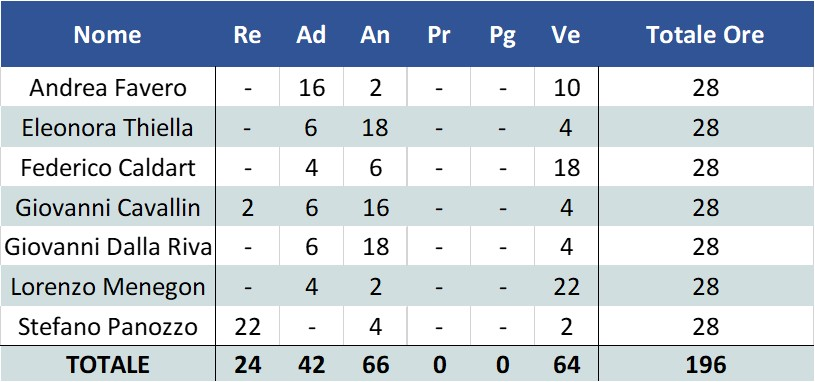
\includegraphics[scale=0.4]{img/Preventivo/AnalisiRequisiti.Orario.jpg}}
	\caption{Prospetto Orario: Analisi dei requisiti}
\end{figure}
La raffigurazione grafica della suddivisione dei ruoli all'interno del gruppo è così rappresentata: 
\begin{figure}[h!]
	\centerline{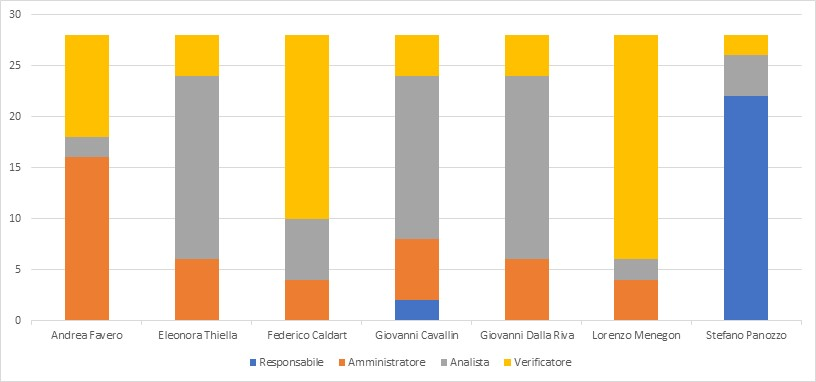
\includegraphics[scale=0.4]{img/Preventivo/Istogrammi/AnalisiRequisiti.jpg}}
	\caption{Raffigurazione Prospetto Orario: Analisi dei requisiti}
\end{figure}
\paragraph{Prospetto economico}
Il prospetto economico per questa attività è illustrato in tabella. Notare che le spese per questa attività non sono a carico del committente.
\begin{figure}[h!]
	\centerline{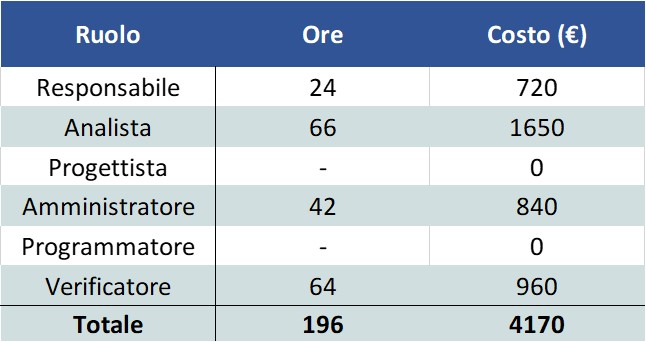
\includegraphics[scale=0.4]{img/Preventivo/AnalisiRequisiti.Economico.jpg}}
	\caption{Prospetto Economico: Analisi dei requisiti}
\end{figure}
La raffigurazione grafica del peso di ogni ruolo sul costo totale è così rappresentata: 
\begin{figure}[h!]
	\centerline{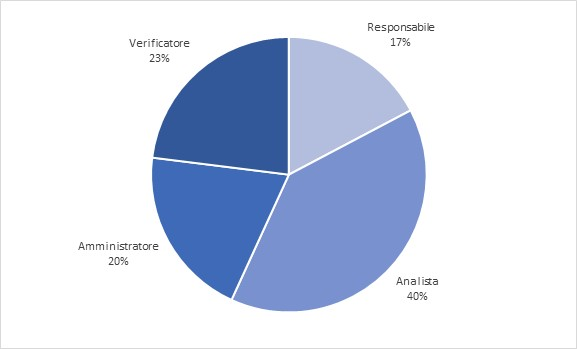
\includegraphics[scale=0.4]{img/Preventivo/Torte/AnalisiRequisiti.jpg}}
	\caption{Raffigurazione Prospetto Economico: Analisi dei requisiti}
\end{figure}

\subsubsection{Analisi dei requisiti in dettaglio}
\paragraph{Prospetto orario}
\begin{figure}[h!]
	\centerline{\includegraphics[scale=0.4]{img/Preventivo/AnalisiRequisitiDettaglio.Orario.jpg}}
	\caption{Prospetto Orario: Analisi dei requisiti in dettaglio}
\end{figure}
La raffigurazione grafica della suddivisione dei ruoli all'interno del gruppo è così rappresentata: 
\begin{figure}[h!]
	\centerline{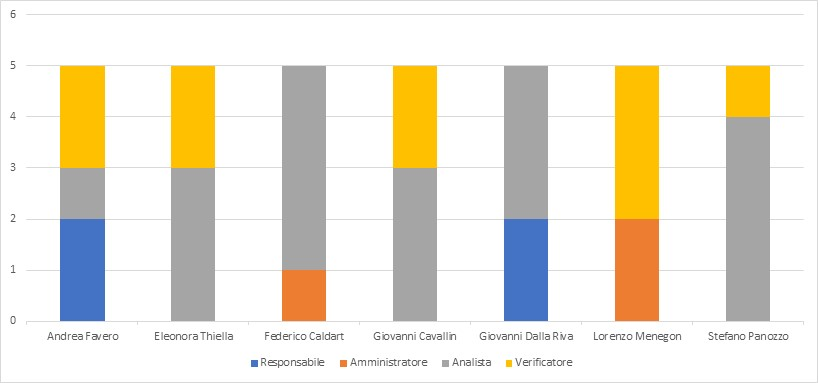
\includegraphics[scale=0.4]{img/Preventivo/Istogrammi/AnalisiRequisitiDettaglio.jpg}}
	\caption{Raffigurazione Prospetto Orario: Analisi dei requisiti in dettaglio}
\end{figure}
\paragraph{Prospetto economico}
Il prospetto economico per questa attività è illustrato in tabella. Notare che le spese per questa attività non sono a carico del committente.
\begin{figure}[h!]
	\centerline{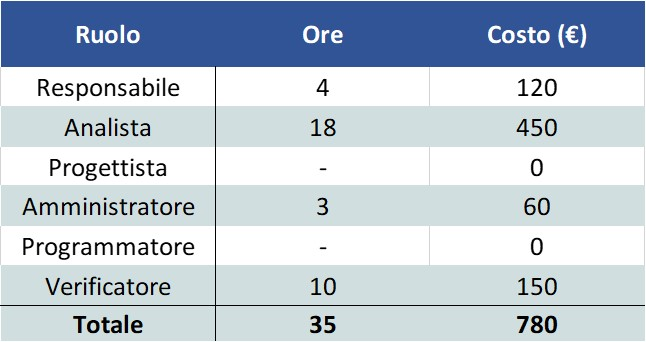
\includegraphics[scale=0.4]{img/Preventivo/AnalisiRequisitiDettaglio.Economico.jpg}}
	\caption{Prospetto Economico: Analisi dei requisiti in dettaglio}
\end{figure}
La raffigurazione grafica del peso di ogni ruolo sul costo totale è così rappresentata: 
\begin{figure}[h!]
	\centerline{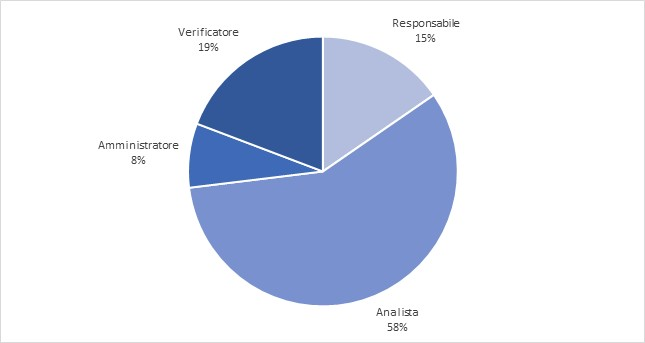
\includegraphics[scale=0.4]{img/Preventivo/Torte/AnalisiRequisitiDettaglio.jpg}}
	\caption{Raffigurazione Prospetto Economico: Analisi dei requisiti in dettaglio}
\end{figure}

\subsection{Attività a carico del committente}
\subsubsection{Prototipazione}
\paragraph{Prospetto orario}
\begin{figure}[h!]
	\centerline{\includegraphics[scale=0.4]{img/Preventivo/Prototipazione.Orario.jpg}}
	\caption{Prospetto Orario: Prototipazione}
\end{figure}
La raffigurazione grafica della suddivisione dei ruoli all'interno del gruppo è così rappresentata: 
\begin{figure}[h!]
	\centerline{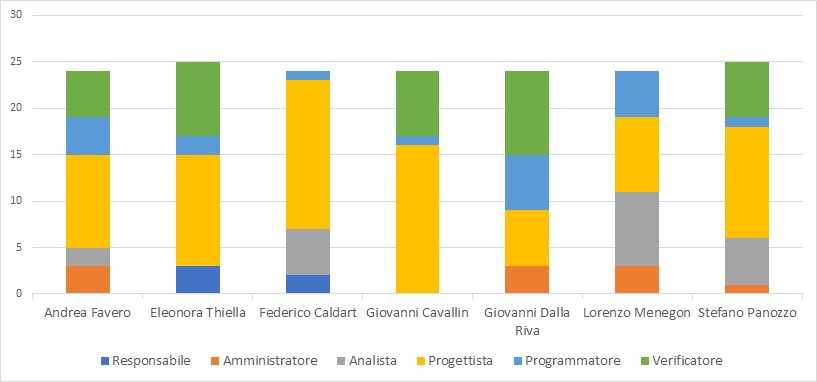
\includegraphics[scale=0.4]{img/Preventivo/Istogrammi/Prototipazione.jpg}}
	\caption{Raffigurazione Prospetto Orario: Prototipazione}
\end{figure}
\paragraph{Prospetto economico}
Il prospetto economico per questa attività è illustrato in tabella. 
\begin{figure}[h!]
	\centerline{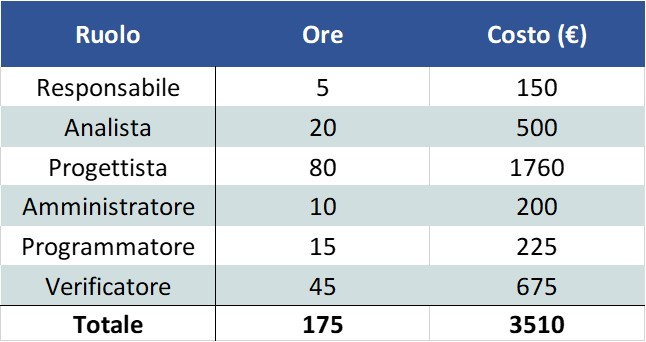
\includegraphics[scale=0.4]{img/Preventivo/Prototipazione.Economico.jpg}}
	\caption{Prospetto Economico: Prototipazione}
\end{figure}
La raffigurazione grafica del peso di ogni ruolo sul costo totale è così rappresentata: 
\begin{figure}[h!]
	\centerline{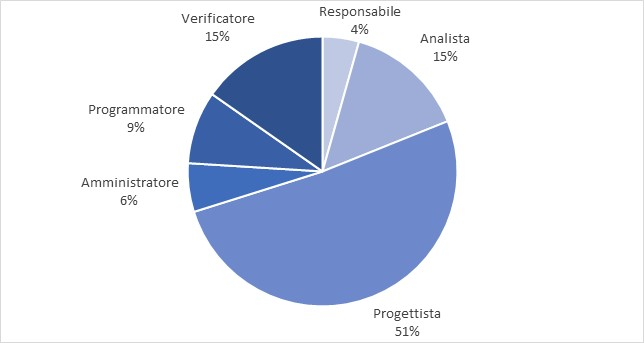
\includegraphics[scale=0.4]{img/Preventivo/Torte/Prototipazione.jpg}}
	\caption{Raffigurazione Prospetto Economico: Prototipazione}
\end{figure}

\subsubsection{Prototipazione in dettaglio}
\paragraph{Prospetto orario}
\begin{figure}[h!]
	\centerline{\includegraphics[scale=0.4]{img/Preventivo/PrototipazioneDettaglio.Orario.jpg}}
	\caption{Prospetto Orario: Prototipazione in dettaglio}
\end{figure}
La raffigurazione grafica della suddivisione dei ruoli all'interno del gruppo è così rappresentata: 
\begin{figure}[h!]
	\centerline{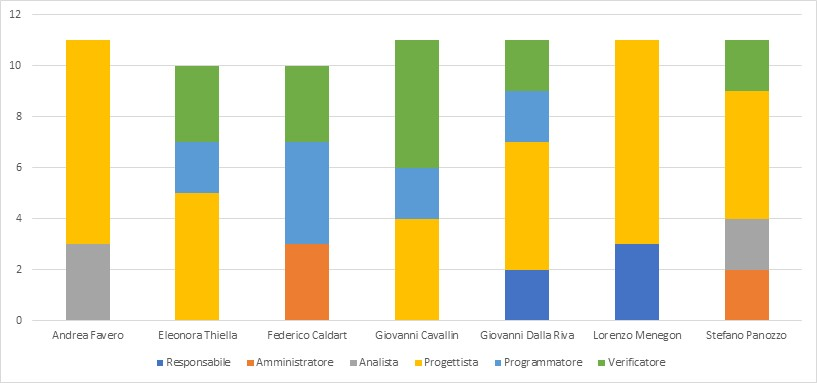
\includegraphics[scale=0.4]{img/Preventivo/Istogrammi/PrototipazioneDettaglio.jpg}}
	\caption{Raffigurazione Prospetto Orario: Prototipazione in dettaglio}
\end{figure}
\paragraph{Prospetto economico}
Il prospetto economico per questa attività è illustrato in tabella. 
\begin{figure}[h!]
	\centerline{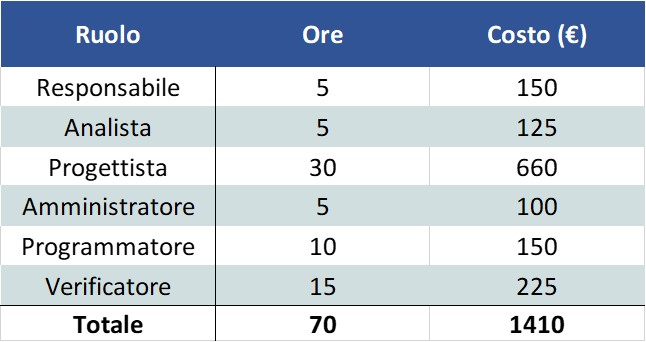
\includegraphics[scale=0.4]{img/Preventivo/PrototipazioneDettaglio.Economico.jpg}}
	\caption{Prospetto Economico: Prototipazione in dettaglio}
\end{figure}
La raffigurazione grafica del peso di ogni ruolo sul costo totale è così rappresentata:
\begin{figure}[h!]
	\centerline{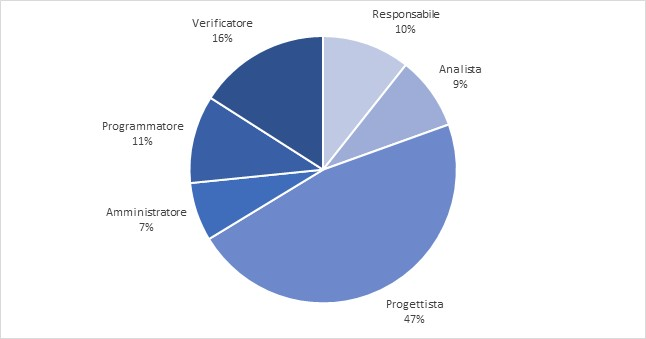
\includegraphics[scale=0.4]{img/Preventivo/Torte/PrototipazioneDettaglio.jpg}}
	\caption{Raffigurazione Prospetto Economico: Prototipazione in dettaglio}
\end{figure} 

\subsubsection{Progettazione finale e Codifica}
\paragraph{Prospetto orario}
\begin{figure}[h!]
	\centerline{\includegraphics[scale=0.4]{img/Preventivo/ProgettazioneFinaleCodifica.Orario.jpg}}
	\caption{Prospetto Orario: Progettazione finale e Codifica}
\end{figure}
La raffigurazione grafica della suddivisione dei ruoli all'interno del gruppo è così rappresentata: 
\begin{figure}[h!]
	\centerline{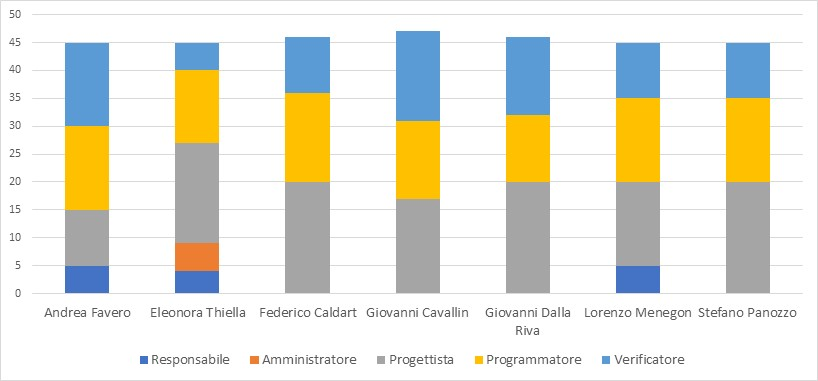
\includegraphics[scale=0.4]{img/Preventivo/Istogrammi/ProgettazioneFinaleCodifica.jpg}}
	\caption{Raffigurazione Prospetto Orario: Progettazione finale e Codifica}
\end{figure}
\paragraph{Prospetto economico}
Il prospetto economico per questa attività è illustrato in tabella. 
\begin{figure}[h!]
	\centerline{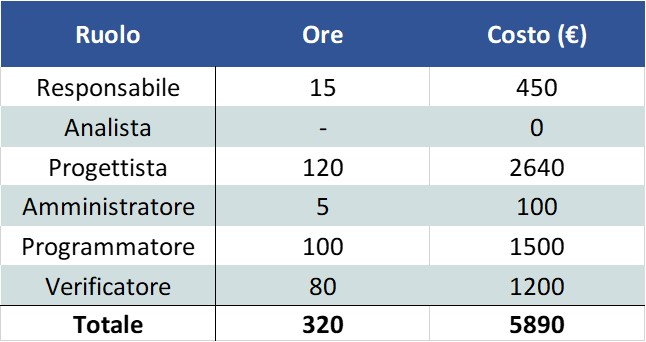
\includegraphics[scale=0.4]{img/Preventivo/ProgettazioneFinaleCodifica.Economico.jpg}}
	\caption{Prospetto Economico: Progettazione finale e Codifica}
\end{figure}
La raffigurazione grafica del peso di ogni ruolo sul costo totale è così rappresentata: 
\begin{figure}[h!]
	\centerline{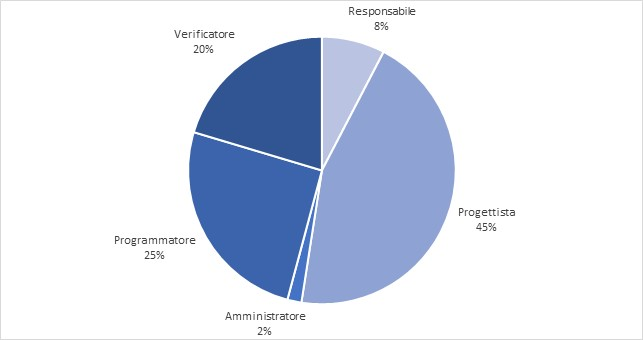
\includegraphics[scale=0.4]{img/Preventivo/Torte/ProgettazioneFinaleCodifica.jpg}}
	\caption{Raffigurazione Prospetto Economico: Progettazione finale e Codifica}
\end{figure} 

\subsubsection{Codifica in dettaglio, Validazione e Collaudo}
\paragraph{Prospetto orario}
\begin{figure}[h!]
	\centerline{\includegraphics[scale=0.4]{img/Preventivo/CodDettaglioValidazioneCollaudo.Orario.jpg}}
	\caption{Prospetto Orario: Codifica in dettaglio, Validazione e Collaudo}
\end{figure}
La raffigurazione grafica della suddivisione dei ruoli all'interno del gruppo è così rappresentata: 
\begin{figure}[h!]
	\centerline{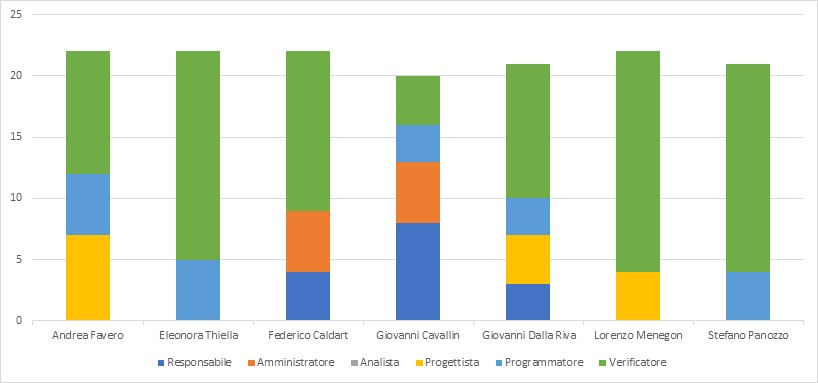
\includegraphics[scale=0.4]{img/Preventivo/Istogrammi/CodDettaglioValidazioneCollaudo.jpg}}
	\caption{Raffigurazione Prospetto Orario: Codifica in dettaglio, Validazione e Collaudo}
\end{figure}
\paragraph{Prospetto economico}
Il prospetto economico per questa attività è illustrato in tabella. 
\begin{figure}[h!]
	\centerline{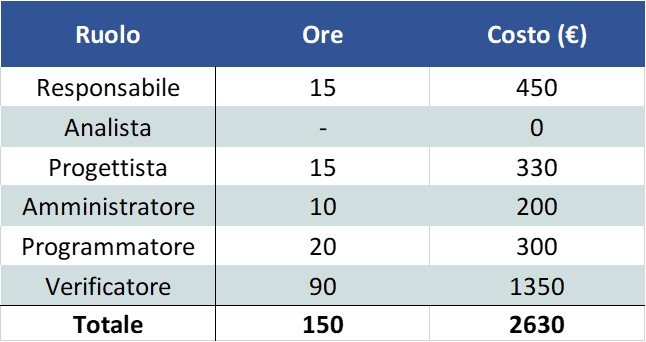
\includegraphics[scale=0.4]{img/Preventivo/CodDettaglioValidazioneCollaudo.Economico.jpg}}
	\caption{Prospetto Economico: Codifica in dettaglio, Validazione e Collaudo}
\end{figure}
La raffigurazione grafica del peso di ogni ruolo sul costo totale è così rappresentata: 
\begin{figure}[h!]
	\centerline{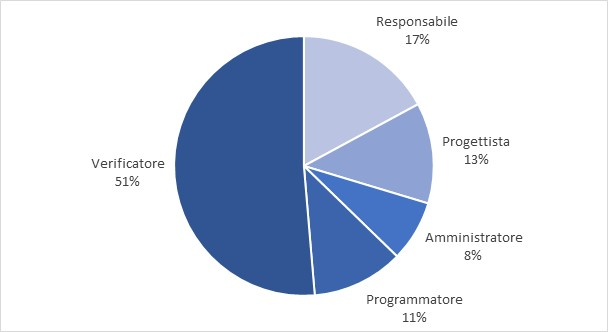
\includegraphics[scale=0.4]{img/Preventivo/Torte/CodDettaglioValidazioneCollaudo.jpg}}
	\caption{Raffigurazione Prospetto Economico: Codifica in dettaglio, Validazione e Collaudo}
\end{figure} 

\subsection{Riepilogo}

\paragraph{Prospetto orario}
In seguito sono presenti il prospetto orario ed economico riepilogativi per tutta la durata del progetto.\\
Si noti la differenza fra le ore totali, comprensive dell'attività di investimento iniziale a carico del gruppo, e le ore rendicontate a carico del committente.
\begin{figure}[h!]
	\centerline{\includegraphics[scale=0.4]{img/Preventivo/ProspettoOreFinale.jpg}}
	\caption{Prospetto Orario: Riepilogo}
\end{figure}
La raffigurazione grafica della suddivisione dei ruoli all'interno del gruppo è così rappresentata: 
\begin{figure}[h!]
	\centerline{\includegraphics[scale=0.4]{img/Preventivo/Istogrammi/ProspettoOreFinale.jpg}}
	\caption{Raffigurazione Prospetto Orario: Riepilogo ore totali}
\end{figure}
\paragraph{Prospetto economico}
\begin{figure}[h!]
	\centerline{\includegraphics[scale=0.4]{img/Preventivo/ProspettoCostoFinale.jpg}}
	\caption{Prospetto Economico: Riepilogo}
\end{figure}
La raffigurazione grafica del peso di ogni ruolo sul costo totale e rendicontato è così rappresentata: 
\begin{figure}[h!]
	\centerline{\includegraphics[scale=0.4]{img/Preventivo/Torte/ProspettoCostoFinaleTotale.jpg}}
	\caption{Raffigurazione Prospetto Economico: Riepilogo ore totali}
\end{figure}
\begin{figure}[h!]
	\centerline{\includegraphics[scale=0.4]{img/Preventivo/Torte/ProspettoCostoFinaleRendicontato.jpg}}
	\caption{Raffigurazione Prospetto Economico: Riepilogo ore rendicontate}
\end{figure}